\documentclass[tikz]{standalone}

\usetikzlibrary{arrows.meta,positioning}

\begin{document}
	\setlength{\baselineskip}{16pt}
	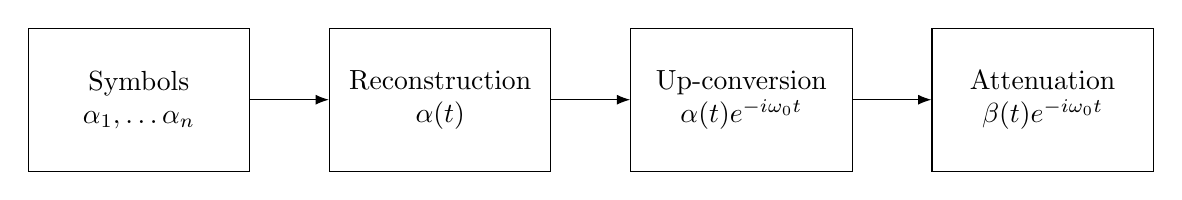
\begin{tikzpicture}[
		block/.style={draw, align=center, minimum height=12ex, minimum width=8em}
	]
		\node[block] (sym) {Symbols\\$\alpha_1,\dots\alpha_n$};
		\node[block, right=of sym] (rec) {Reconstruction\\$\alpha(t)$};
		\node[block, right=of rec] (up) {Up-conversion\\$\alpha(t)e^{-i\omega_0t}$};
		\node[block, right=of up] (att) {Attenuation\\$\beta(t)e^{-i\omega_0t}$};

		\draw[-Latex] (sym) -- (rec);
		\draw[-Latex] (rec) -- (up);
		\draw[-Latex] (up) -- (att);
	\end{tikzpicture}
\end{document}